%%
%% Copyright 2007, 2008, 2009 Elsevier Ltd
%%
%% This file is part of the 'Elsarticle Bundle'.
%% ---------------------------------------------
%%
%% It may be distributed under the conditions of the LaTeX Project Public
%% License, either version 1.2 of this license or (at your option) any
%% later version.  The latest version of this license is in
%%    http://www.latex-project.org/lppl.txt
%% and version 1.2 or later is part of all distributions of LaTeX
%% version 1999/12/01 or later.
%%
%% The list of all files belonging to the 'Elsarticle Bundle' is
%% given in the file `manifest.txt'.
%%

%% Template article for Elsevier's document class `elsarticle'
%% with numbered style bibliographic references
%% SP 2008/03/01
%%
%%
%%
%% $Id: elsarticle-template-num.tex 4 2009-10-24 08:22:58Z rishi $
%%
%%
\documentclass[preprint,12pt]{elsarticle}

%% Use the option review to obtain double line spacing
%% \documentclass[preprint,review,12pt]{elsarticle}

%% Use the options 1p,twocolumn; 3p; 3p,twocolumn; 5p; or 5p,twocolumn
%% for a journal layout:
%% \documentclass[final,1p,times]{elsarticle}
%% \documentclass[final,1p,times,twocolumn]{elsarticle}
%% \documentclass[final,3p,times]{elsarticle}
%% \documentclass[final,3p,times,twocolumn]{elsarticle}
%% \documentclass[final,5p,times]{elsarticle}
%% \documentclass[final,5p,times,twocolumn]{elsarticle}

%% if you use PostScript figures in your article
\usepackage{url}
%% use the graphics package for simple commands
\usepackage{graphics}
%% or use the graphicx package for more complicated commands
\usepackage{graphicx}
%% or use the epsfig package if you prefer to use the old commands
%% \usepackage{epsfig}
%%\usepackage{pifont}%use circled number
\usepackage{booktabs}
\usepackage{longtable}
\usepackage{multirow}
\usepackage{subfig}
%% The amssymb package provides various useful mathematical symbols
\usepackage{amssymb}
%% The amsthm package provides extended theorem environments
%% \usepackage{amsthm}

%% The lineno packages adds line numbers. Start line numbering with
%% \begin{linenumbers}, end it with \end{linenumbers}. Or switch it on
%% for the whole article with \linenumbers after \end{frontmatter}.
%% \usepackage{lineno}

%% natbib.sty is loaded by default. However, natbib options can be
%% provided with \biboptions{...} command. Following options are
%% valid:

%%   round  -  round parentheses are used (default)
%%   square -  square brackets are used   [option]
%%   curly  -  curly braces are used      {option}
%%   angle  -  angle brackets are used    <option>
%%   semicolon  -  multiple citations separated by semi-colon
%%   colon  - same as semicolon, an earlier confusion
%%   comma  -  separated by comma
%%   numbers-  selects numerical citations
%%   super  -  numerical citations as superscripts
%%   sort   -  sorts multiple citations according to order in ref. list
%%   sort&compress   -  like sort, but also compresses numerical citations
%%   compress - compresses without sorting
%%
%% \biboptions{comma,round}

% \biboptions{}

%\journal{Nuclear Physics B}

\begin{document}

\begin{frontmatter}

%% Title, authors and addresses

%% use the tnoteref command within \title for footnotes;
%% use the tnotetext command for the associated footnote;
%% use the fnref command within \author or \address for footnotes;
%% use the fntext command for the associated footnote;
%% use the corref command within \author for corresponding author footnotes;
%% use the cortext command for the associated footnote;
%% use the ead command for the email address,
%% and the form \ead[url] for the home page:
%%
%% \title{Title\tnoteref{label1}}
%% \tnotetext[label1]{}
%% \author{Name\corref{cor1}\fnref{label2}}
%% \ead{email address}
%% \ead[url]{home page}
%% \fntext[label2]{}
%% \cortext[cor1]{}
%% \address{Address\fnref{label3}}
%% \fntext[label3]{}

\title{Multi-path Partial Scintillator Fitter}

%% use optional labels to link authors explicitly to addresses:
%% \author[label1,label2]{<author name>}
%% \address[label1]{<address>}
%% \address[label2]{<address>}

\author{Aksel Hallin, David Auty, Kalpana Singh, Jeff Tseng, Jie Hu}

\address{University of Alberta}

\begin{abstract}
 Multi-path partial fitter

\end{abstract}

\begin{keyword}
%% keywords here, in the form: keyword \sep keyword
Multi-path fitter \sep partial fitter \sep scintillator
%% MSC codes here, in the form: \MSC code \sep code
%% or \MSC[2008] code \sep code (2000 is the default)

\end{keyword}

\end{frontmatter}

%%
%% Start line numbering here if you want
%%
% \linenumbers

%% main text
\section{Fitter ideas}


\section{Likelihood functions}
\textbf{Notations}

time of flight: $t_{tof}$

time residue: $t_{res}$

refraction index of water: $n_w$

refraction index of scintillator: $n_s$

$L$: water level (z value of the water level in the AV coordinate)

vertex(trial) position: $\vec{X}_{V} = (X_0, Y_0, Z_0)$

trial time: $t_0$

PMT position: $\vec{X}_{P} = (X_P, Y_P, Z_P)$

$fD$: vertex depth, depth of vertex below the water level, $fD = L - Z_0$

$fH$: PMT height, height of PMT above the water level, $fH = Z_P - L$ 

$\alpha$: fractional factor of the transverse distance between water-vertex intersection

$\vec{I}$: incident light vector, pointing from the vertex point to incident point in the water-scintillator interface   

$\vec{R}$: reflected light vector

$P_R$: reflection probability, calculated by interpolating Fresnel equation

$\vec{T}$: transmitted(or refracted) light vector

$\vec{S}$: intersection vector for calculating $\vec{R},~\vec{T}$


Fresnel equation: 
$n_t$, $\theta_t$, $n_i$, $\theta_t$, and $\cos\theta_t=\sqrt{1-\frac{n_i}{n_t}\sin^2\theta_i}$

\[
R_P = \left|\frac{n_t\cos\theta_i - n_i\cos\theta_t}{n_t\cos\theta_i+n_i\cos\theta_t}\right|^2
\]

\[
R_S = \left|\frac{n_i\cos\theta_i - n_t\cos\theta_t}{n_i\cos\theta_i+n_t\cos\theta_t}\right|^2
\]


Different cases are classified by the layouts of vertex and PMT positions. 
\begin{itemize}
\item Vertex below water level, PMT below water level
\item Vertex below water level, PMT above water level
\item Vertex above water level, PMT below water level
\item Vertex above water level, PMT above water level
\end{itemize}

\subsection{Vertex below water level, PMT below water level}
In this case we consider two light paths: direct light path and reflected light path.

$\alpha = sD/(sD-fH)$, 

$\vec{S} = (1-\alpha)\vec{X}_V+\alpha\vec{X}_P$, and then set $S_z = L$. As shown in figure, 
$\vec{I}$ and $\vec{R}$ can be calculated as:

$\vec{I} = \vec{S}-\vec{X}_V$, $\vec{R} = \vec{X}_P-\vec{S}$ 

For direct light path, $t_{tof,direct} = |\vec{X}_{V}-\vec{X}_{P}|/(c/n_w),~t_{res,direct} = t_{PMT} - t_{tof,direct} - t_0$

For reflected light path, $t_{tof,refl} = (|\vec{I}|+|\vec{R}|)/(c/n_w)$

The reflection probability $P_R$

The likelihood function is:
\[
L = L_{Ch}(t_{tof,direct}) + P_R L_{Ch}(t_{tof,refl})
\]
\[
\frac{dL}{dx} = \frac{dL}{dt_{tof}}\frac{t_{tof}}{dx}
\]
\[
\frac{dL}{dt} = \frac{dL}{dt_{tof}}
\]

\begin{figure}[htbp]
	\centering	
	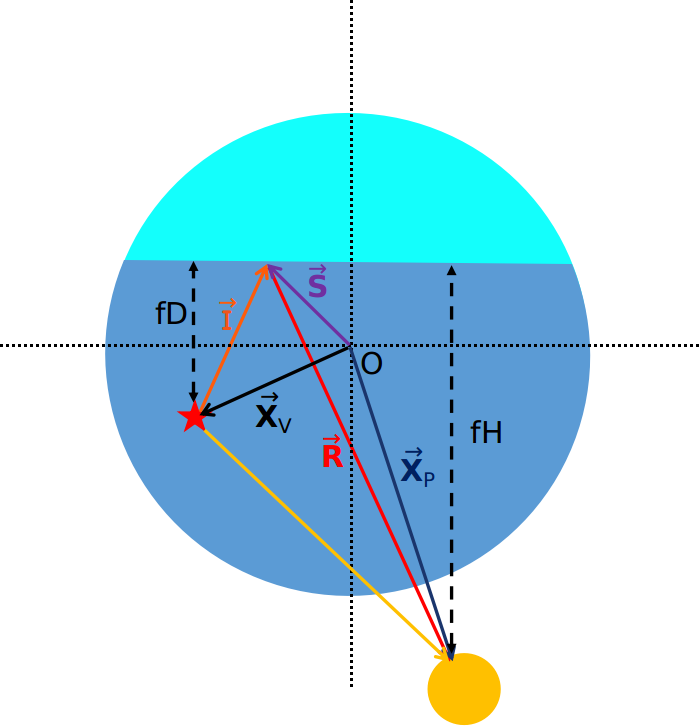
\includegraphics[width=6cm]{geo_VbPb.png}
	\caption{\label{VbPb} 
	Layout of event when both vertex and PMT are below the water level.
	}
\end{figure}



\subsection{Vertex below water level, PMT above water level}




\begin{figure}[htbp]
	\centering	
	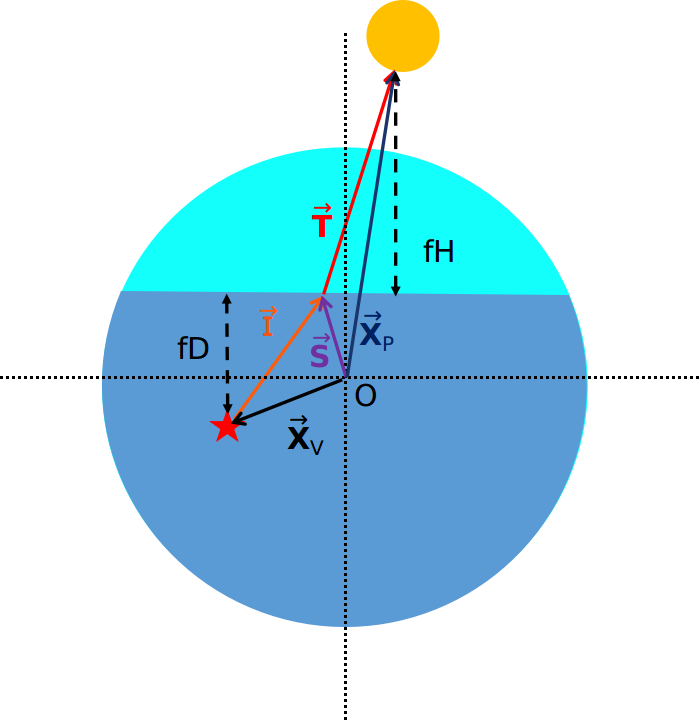
\includegraphics[width=6cm]{geo_VbPt.png}
	\caption{\label{VbPt} 
		Layout of the event when vertex is below the water level and PMT is above.
	}
\end{figure}


\subsection{Vertex above water level, PMT below water level}

$\alpha = sD/(sD-fH)$, 

$\vec{S} = (1-\alpha)\vec{X}_V+\alpha\vec{X}_P$, and then set $S_z = L$. As shown in figure, 
$\vec{I}$ and $\vec{R}$ can be calculated as:

$\vec{I} = \vec{S}-\vec{X}_V$, $\vec{T} = \vec{X}_P-\vec{S}$, 



\begin{figure}[htbp]
	\centering	
	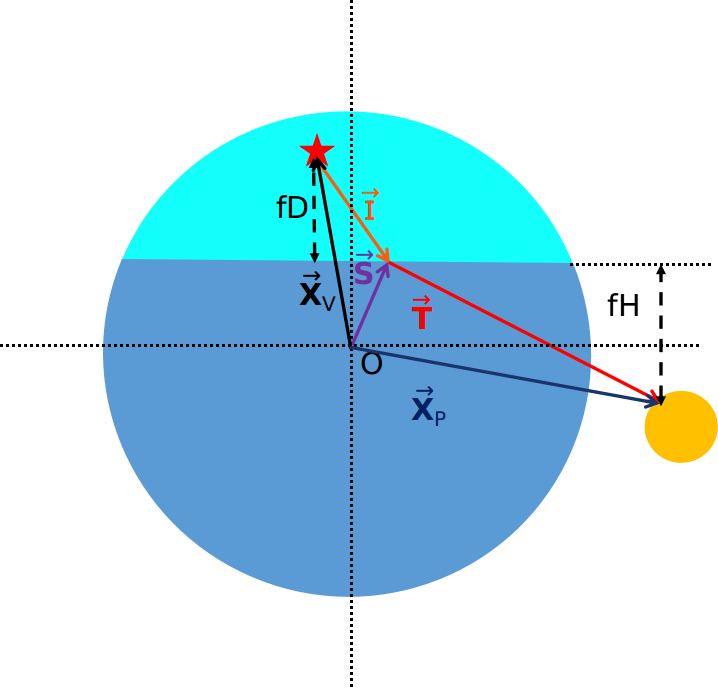
\includegraphics[width=6cm]{geo_VtPb.png}
	\caption{\label{VtPb} 
		Layout of the event when vertex is above the water level and PMT is below.
	}
\end{figure}

\subsection{Vertex above water level, PMT babove water level}




\begin{figure}[htbp]
	\centering	
	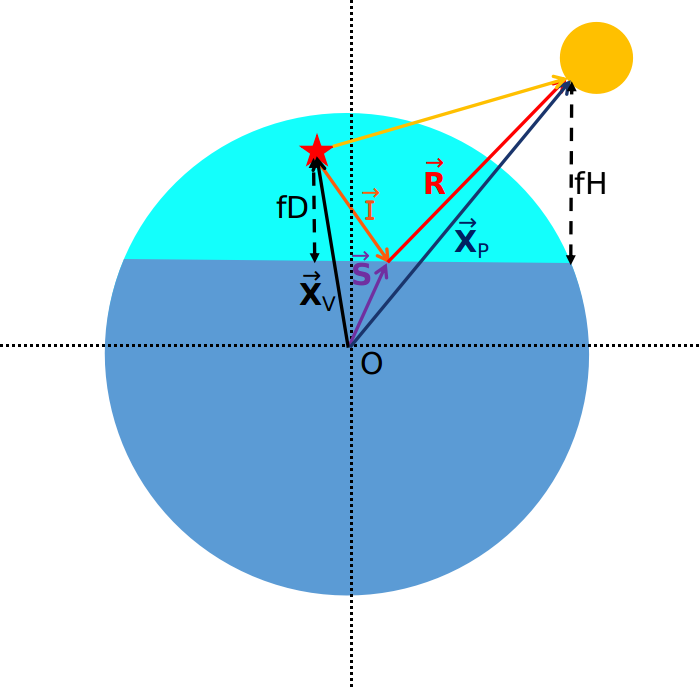
\includegraphics[width=6cm]{geo_VtPt.png}
	\caption{\label{VtPt} 
		Layout of the event when both vertex and PMT are above the water level.
	}
\end{figure}



\section{Monte Carlo Results}


\section{Conclusions}


\vspace{30mm}
\bibliographystyle{elsarticle-num}
\bibliography{<your-bib-database>}

%% Authors are advised to submit their bibtex database files. They are
%% requested to list a bibtex style file in the manuscript if they do
%% not want to use elsarticle-num.bst.

%% References without bibTeX database:

\begin{thebibliography}{00}

%% \bibitem must have the following form:
%%   \bibitem{key}...
\bibitem{Aksel}  

\end{thebibliography}


\end{document}

%%
%% End of file `elsarticle-template-num.tex'.
